\subsubsection{Versuch: Bestätigung der hohen Lichtdurchlässigkeit von PC und der einfachen Weiterverarbeitung}

Material:
\begin{itemize*}
    \item handelsübliche CD, Schere, 2 Glasschalen, Plätzchenform, Pinzette, Alufolie, Heizplatte
    \item Chemikalien: Salpetersäure (Sicherheitshinweis: CAS Nr. 7697-37-2; Oxidierende Flüssigkeiten, Kategorie 2 (siehe \autoref{fig:cdbrandfoerdernd}); Ätzwirkung auf die Haut, Kategorie 1A (siehe \autoref{fig:cdaetzwirkung}))
\end{itemize*}

\begin{figure}[h]
    \begin{center}
        \begin{minipage}[t]{0.4\textwidth}
            \begin{center}
                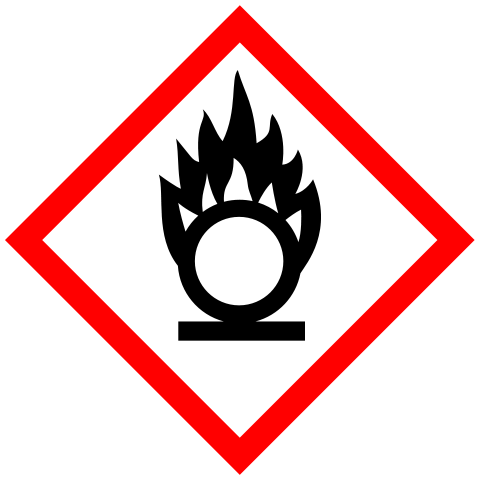
\includegraphics[height=0.1\textheight]{Bilder/Optische_Datentraeger_Die_Compact_Disc/Material_Polycarbonat/cdbrandfoerdernd.png}
                \caption[Oxidierende Flüssigkeiten, Kategorie 2 \newline \url{https://upload.wikimedia.org/wikipedia/commons/e/e5/GHS-pictogram-rondflam.svg}]{Oxidierende Flüssigkeiten, Kategorie 2}
                \label{fig:cdbrandfoerdernd}
            \end{center}
        \end{minipage}
        \hspace{0.025\textwidth}
        \begin{minipage}[t]{0.4\textwidth}
            \begin{center}
                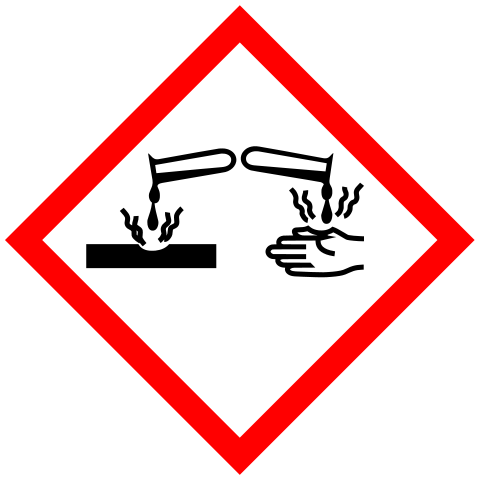
\includegraphics[height=0.1\textheight]{Bilder/Optische_Datentraeger_Die_Compact_Disc/Material_Polycarbonat/cdaetzwirkung.png}
                \caption[Ätzwirkung auf die Haut, Kategorie 1A \newline \url{https://upload.wikimedia.org/wikipedia/commons/a/a1/GHS-pictogram-acid.svg}]{Ätzwirkung auf die Haut, Kategorie 1A}
                \label{fig:cdaetzwirkung}
            \end{center}
        \end{minipage}
    \end{center}
\end{figure}

Schutzvorkehrungen:
\begin{itemize}
    \item Abzug, Kittel, Handschuhe, Schutzbrille
\end{itemize}

Versuchsablauf:
\begin{enumerate*}
    \item Die CD wird in eine der Glasschalen gelegt und mit Salpetersäure übergossen (siehe \autoref{fig:cdsalpeter}). Dies muss unter einem Abzug geschehen, da nitrose Gase entstehen.
    \item Nach kurzer Zeit \shorthandoff{"}"quillt"\shorthandon{"} die Lack- und die Aluminiumschicht auf (siehe \autoref{fig:cdquillt}) und lässt sich mithilfe der Pinzette entfernen.
    \item Die \shorthandoff{"}"gehäutete"\shorthandon{"} CD wird nun in die zweite Glasschale gelegt und vorsichtig unter dem Wasserhahn abgespült. \autoref{fig:cdblank} zeigt die resultierende Polycarbonatscheibe. \footnote{Zu diesem Zeitpunkt kann die erste Behauptung überprüft werden.}
    %TODO: Sicherheitshinweis Wasser auf Säure.
    \item Die Polycarbonatscheibe wird nun in kleine Stücke zerschnitten, die nicht größer als 1 cm² sind (siehe \autoref{fig:cdzerschnitten})
    \item Die Polycarbonatschnipsel werden ca. 1 cm hoch in die Plätzchenform gegeben, welche sich auf der mit Aluminiumfolie bedeckten Heizplatte befindet. %TODO: Bild Heizplatte
    \item Die Heizplatte wird auf über 250°C und man wartet bis das Polycarbonat zu einer gleichmäßigen Oberfläche zerflossen ist.
    \item Die Heizplatte wird nun ausgeschalten und das \shorthandoff{"}"Polycarbonatplätzchen"\shorthandon{"} kann aus seiner Form gebrochen werden, sobald diese abgekühlt ist. %TODO: Bild von Polycarbonatplätzchen
\end{enumerate*}

\begin{figure}[h]
    \begin{center}
        \begin{minipage}[t]{0.4\textwidth}
            \begin{center}
                \includegraphics[height=0.1\textheight]{Bilder/Optische_Datentraeger_Die_Compact_Disc/Material_Polycarbonat/cdsalpeter.png}
                \caption[CD in Salpetersäure]{CD in Salpetersäure}
                \label{fig:cdsalpeter}
            \end{center}
        \end{minipage}
        \hspace{0.025\textwidth}
        \begin{minipage}[t]{0.4\textwidth}
            \begin{center}
                \includegraphics[height=0.1\textheight]{Bilder/Optische_Datentraeger_Die_Compact_Disc/Material_Polycarbonat/cdquillt.png}
                \caption[\shorthandoff{"}"\shorthandon{"}\shorthandoff{"}Aufgequollene"\shorthandon{"} Lack- und Aluminiumschicht]{\shorthandoff{"}"\shorthandon{"}\shorthandoff{"}Aufgequollene"\shorthandon{"} Lack- und Aluminiumschicht}
                \label{fig:cdquillt}
            \end{center}
        \end{minipage}
    \end{center}

    \begin{center}
        \begin{minipage}[t]{0.4\textwidth}
            \begin{center}
                \includegraphics[height=0.1\textheight]{Bilder/Optische_Datentraeger_Die_Compact_Disc/Material_Polycarbonat/cdblank.png}
                \caption[Polycarbonatscheibe]{Polycarbonatscheibe}
                \label{fig:cdblank}
            \end{center}
        \end{minipage}
        \hspace{0.025\textwidth}
        \begin{minipage}[t]{0.4\textwidth}
            \begin{center}
                \includegraphics[height=0.1\textheight]{Bilder/Optische_Datentraeger_Die_Compact_Disc/Material_Polycarbonat/cdzerschnitten.png}
                \caption[CD in kleine Stücke zerschnitten]{CD in kleine Stücke zerschnitten}
                \label{fig:cdzerschnitten}
            \end{center}
        \end{minipage}
    \end{center}
\end{figure}

Behauptungen: %TODO: Bessere Bezeichnung
\begin{enumerate*}
    \item hohe Lichtdurchlässigkeit: Wenn man die Polycarbonatscheibe in das CD-Laufwerk eines Computers einlegt, erkennt dieser nicht das eine CD eingelegt wurde, da der Laserstrahl ungehindert durch die Polycarbonatscheibe geht. Dies beweist ebenfalls, dass die Aluminiumschicht für die Reflektion des Laserstrahls verantwortlich ist.
    \item einfache Weiterverarbeitung: Die Polycarbonatschnipsel lassen sich ohne großen Aufwand und innerhalb kurzer Zeit in eine neue Form schmelzen. Die Qualitätsminderung liegt an den Verschmutzungen, die aufgrund der primitiven Methoden sich nicht vermeiden lässt.
\end{enumerate*}
